\section{Issuer}

\subsection{Registrazione}
In questa sezione un utente può registarsi inserendo \textit{Email} e \textit{Password} valide. Una volta registrato l'utente riceverà un messaggio di conferma e verrà reindirizzato alla pagina \textit{Home}.
\begin{center}
\includegraphics[scale = 0.2]{./res/img/issuer/registrazione/registrazione1.png}
\includegraphics[scale = 0.2]{./res/img/issuer/registrazione/registrazione2.png}
\includegraphics[scale = 0.2]{./res/img/issuer/registrazione/registrazione3.png}
\end{center}

\subsection{Login}
\subsubsection{Login utente}
In questa pagina un \textbf{utente} può effettuare il login inserendo \textit{Email} e \textit{Password} valide. Una volta effettuato il login l'utente verrà reindirizzato alla sua pagina \textit{Home}.
\begin{center}
\includegraphics[scale = 0.2]{./res/img/issuer/login/user/login1.png}
\includegraphics[scale = 0.2]{./res/img/issuer/login/user/login2.png}
\includegraphics[scale = 0.2]{./res/img/issuer/login/user/login3.png}    
\end{center}


\subsubsection{Login admin}
In questa pagina un \textbf{admin} può effettuare il login inserendo \textit{Email} e \textit{Password} valide. Una volta effettuato il login l'admin verrà reindirizzato alla sua pagina \textit{Home}.
\begin{center}
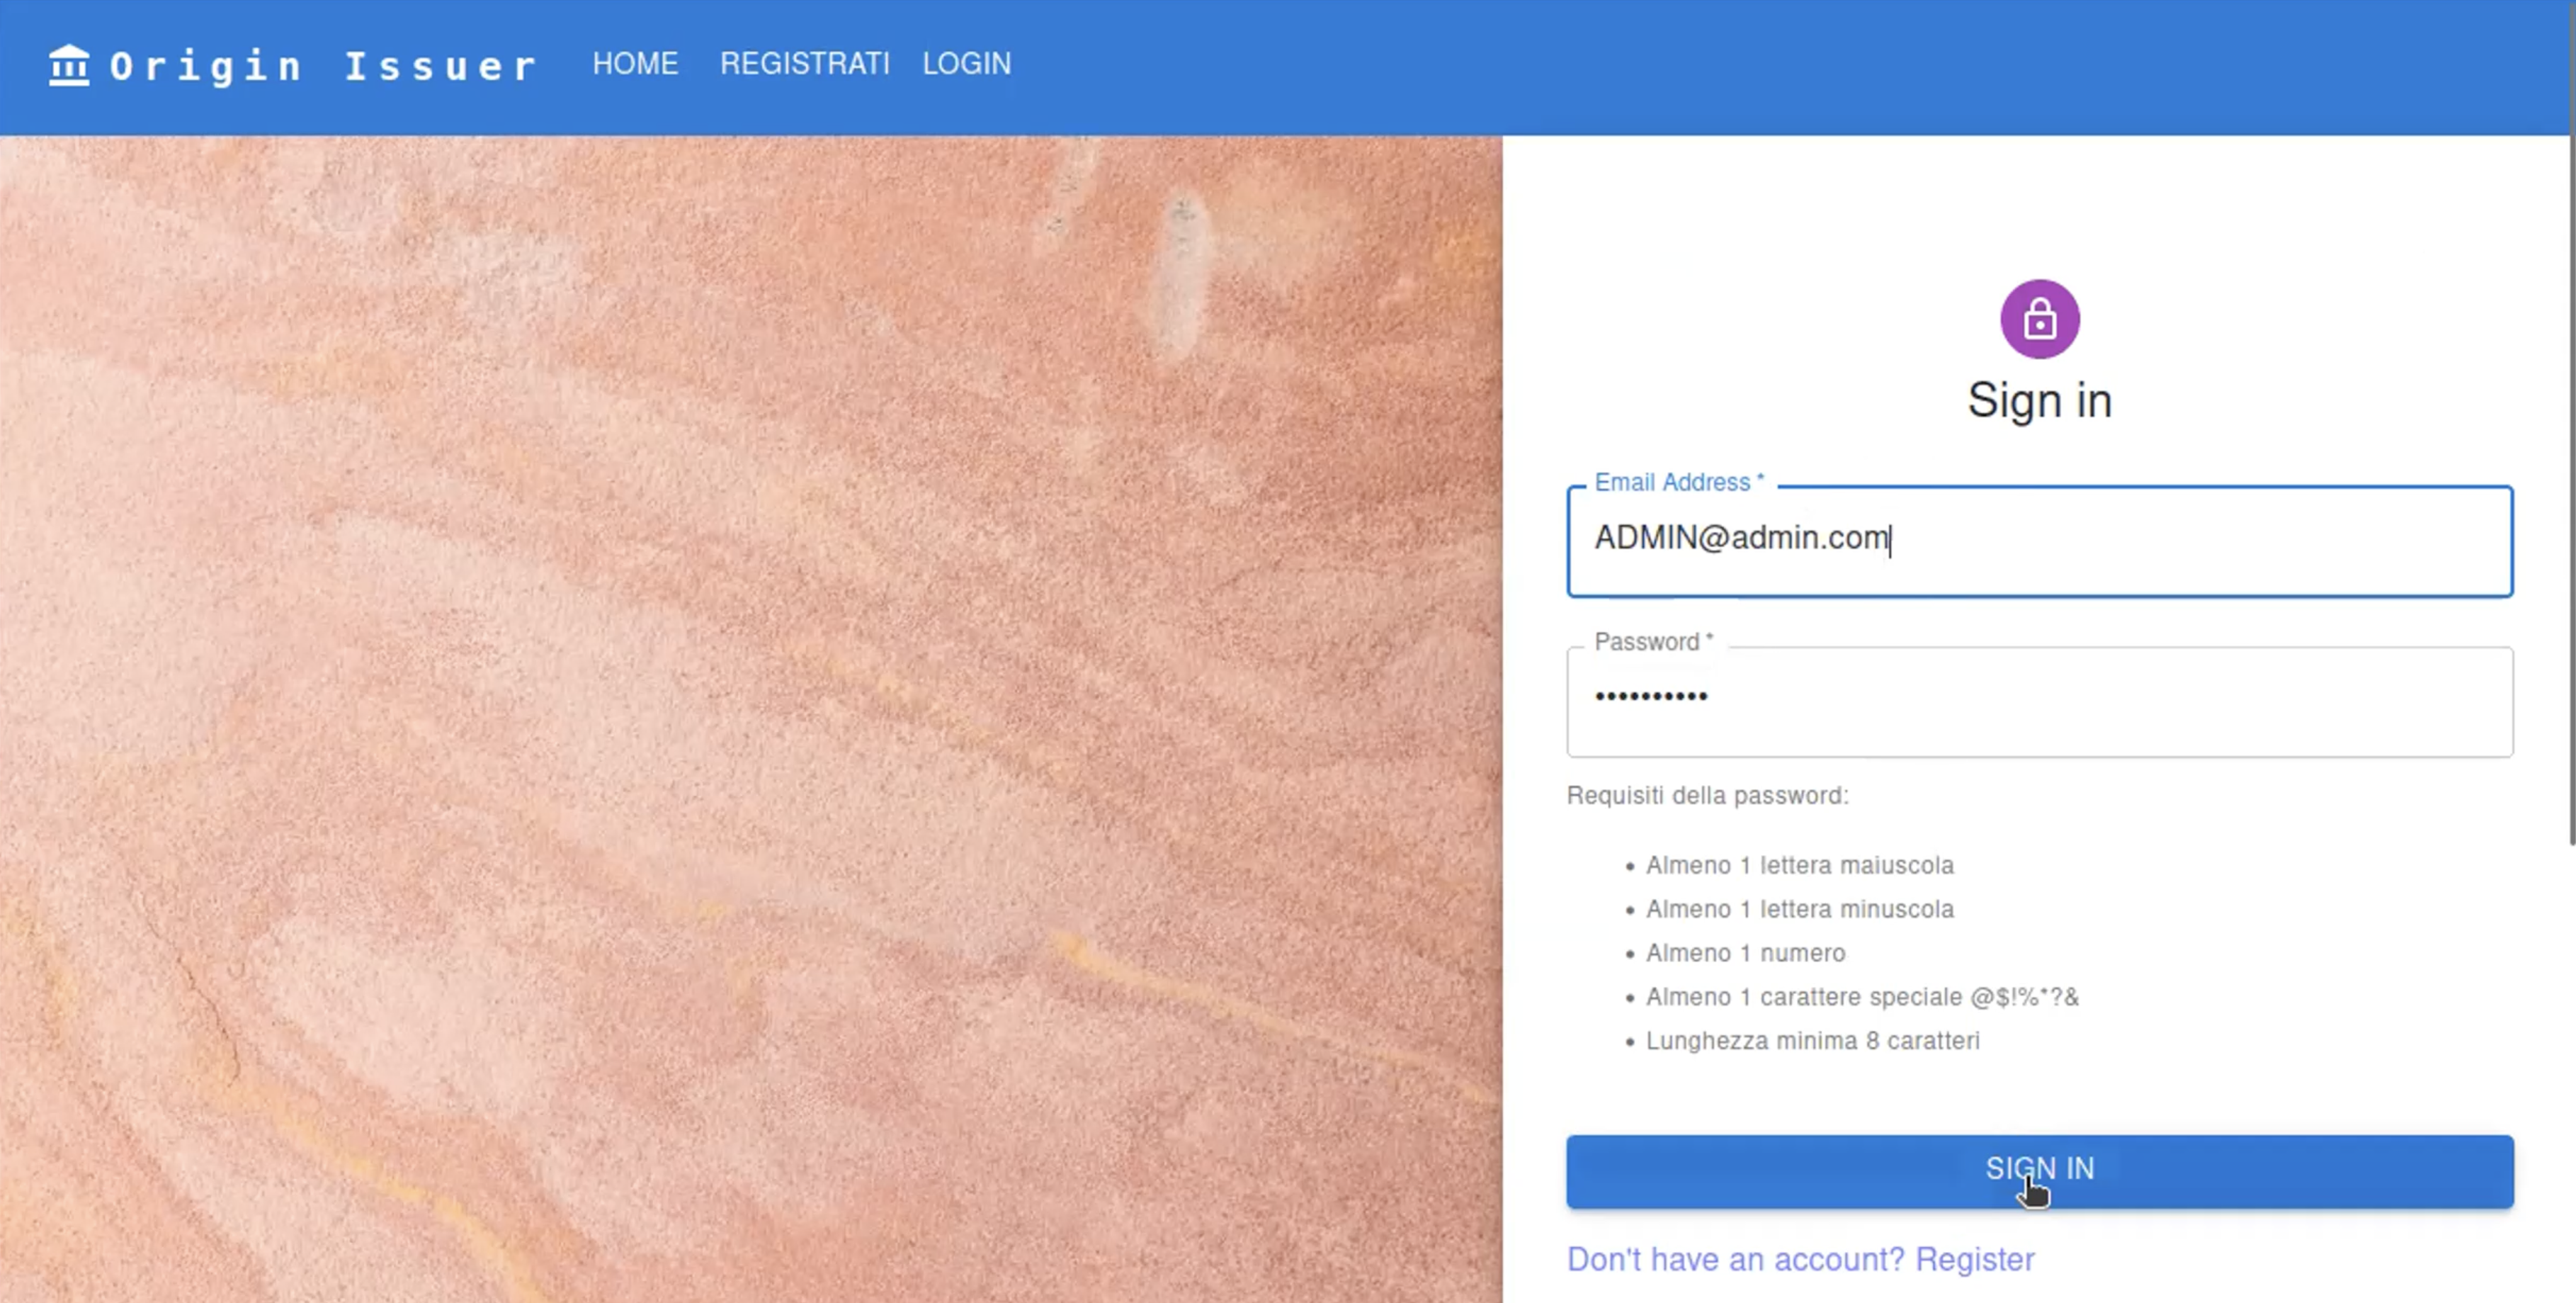
\includegraphics[scale = 0.2]{./res/img/issuer/login/admin/loginAdmin1.png}
\includegraphics[scale = 0.2]{./res/img/issuer/login/admin/loginAdmin2.png}
\includegraphics[scale = 0.2]{./res/img/issuer/login/admin/loginAdmin3.png}
\end{center}

\subsection{Richiesta Credenziale}
\subsubsection{Richiesta PID}
In questa pagina un utente può richiedere una credenziale di tipo \textit{PID} inserendo i dati richiesti. Una volta inseriti i dati l'utente riceverà un messaggio di conferma.
\begin{center}
\includegraphics[scale = 0.2]{./res/img/issuer/richiestaPID/richiestaPID1.png}
\includegraphics[scale = 0.2]{./res/img/issuer/richiestaPID/richiestaPID2.png} 
\includegraphics[scale = 0.2]{./res/img/issuer/richiestaPID/richiestaPID3.png}
\end{center}

\subsubsection{Richiesta Marital Status}
In questa pagina un utente può richiedere una credenziale di tipo \textit{Marital} inserendo i dati richiesti. Una volta inseriti i dati l'utente riceverà un messaggio di conferma.

\subsection{Visualizzazione lista richieste}
\subsubsection{Visualizzazione richieste user} 
In questa pagina l'utente dopo aver fatto una richiesta di credenziale può visualizzare due liste suddivise in PID e Marital con lo stato in cui si trovano. 
Una volta approvata una credenziale si potranno vedere i dettagli di essa.
\begin{center}
\includegraphics[scale = 0.2]{./res/img/issuer/lista/user/listaUser1.png}
\includegraphics[scale = 0.2]{./res/img/issuer/lista/user/listaUser2.png}
\includegraphics[scale = 0.2]{./res/img/issuer/lista/user/listaUser3.png}
\end{center}

\subsubsection{Visualizzazione richieste admin e approvazione} 
In questa pagina un admin può visualizzare due liste suddivise in PID e Marital con lo stato in cui si trovano (da revisionare, revisionate). Cliccando su una 
delle credenziali da revisionare potrà vedere i dettagli e scegliere se approvare o rifiutare la credenziale.
\begin{center}
\includegraphics[scale = 0.2]{./res/img/issuer/lista/admin/listaAdmin1.png}
\includegraphics[scale = 0.2]{./res/img/issuer/lista/admin/listaAdmin2.png}    
\end{center}

\clearpage

\subsection{Rilascio credenziale}
Qunado un utente si trova nella pagina di dettaglio di una sua credenziale potra segliere come rilasciarla: tramite QR code, tramite url oppure tramite un 
pulsante che lo reindirizzerà nel Wallet scelto.
\begin{center}
\includegraphics[scale = 0.2]{./res/img/issuer/rilascio/rilascio1.png}    
\end{center}

